\documentclass{article}

\usepackage[polish]{babel}
\usepackage[utf8]{inputenc}
\usepackage[T1]{fontenc}
\usepackage{amsmath, amssymb, subcaption}

\usepackage[letterpaper,top=2cm,bottom=2cm,left=3cm,right=3cm,marginparwidth=1.75cm]{geometry}
\usepackage{graphicx}

\usepackage{amsmath}
\usepackage{graphicx}
\usepackage[colorlinks=true, allcolors=blue]{hyperref}

\title{Rozwiązywanie układu równań liniowych \(Ax = b\), gdzie \(A(n \times n)\) jest macierzą symetryczną dodatnio określoną}
\author{Kornel Tłaczała}

\begin{document}
\maketitle

\vspace{0.2cm}
\begin{center}
\textbf{\large Projekt nr 2} \\
\end{center}

\section{Opis probelmu}
    \subsection*{Cel projektu}
Niech \(A \in \mathbb{R}^{n \times n} \) będzie dodatnio określoną macierzą symetryczną postaci:
\[
A=\begin{bmatrix}
    A_{11} & A_{12}\\
    A_{12}^T & A_{22}
\end{bmatrix},
\quad A_{ij} \in \mathbb{R}^{p \times p} \quad \wedge \quad n=2p
\]
Zadaniem jest rozwiązać układ równań liniowych \(Ax = b\) korzystając z blokowego rozkładu \(UDU^T\) macierzy \(A\) (\(A = UDU^T\)).
    \subsection*{Metoda rozwiązania}
     \subsubsection*{Szukanie macierzy U i D}
Jeżeli przyjmiemy, że U jest macierzą o postaci:
\[
    U=\begin{bmatrix}
        I & U_{12}\\
        0 & I
    \end{bmatrix}
\]
oraz D jest macierzą o postaci:
\[
    D=\begin{bmatrix}
        D_{11} & 0\\
        0 & D_{22}
    \end{bmatrix}
\]
to zgodnie ze schematem mnożenia macierzy blokowych otrzymujemy:
\[
    A = UDU^T
\]
\vspace{5pt}
\[
    \begin{bmatrix}
        A_{11} & A_{12}\\
        A_{12}^T & A_{22}
    \end{bmatrix}
    =
    \begin{bmatrix}
        I & U_{12}\\
        0 & I
    \end{bmatrix}
    \cdot
    \begin{bmatrix}
        D_{11} & 0\\
        0 & D_{22}
    \end{bmatrix}
    \cdot
    \begin{bmatrix}
        I & 0\\
        U_{12}^T & I
    \end{bmatrix}
    =
\]
\[
=
    \begin{bmatrix}
        D_{11} & U_{12} \cdot D_{22}\\
        0 & D_{22}
    \end{bmatrix}
    \cdot
    \begin{bmatrix}
        I & 0\\
        U_{12}^T & I
    \end{bmatrix}
    =
\]
\[
    =
    \begin{bmatrix}
        D_{11} + U_{12} \cdot D_{22} \cdot U_{12}^T & U_{12} \cdot D_{22}\\
        D_{22} \cdot U_{12}^T & D_{22}
    \end{bmatrix}
\]
Na tej podstawie łatwo będzie znaleźć macierze \(U\) oraz \(D\) za pomocą następującego układu równań, wyznaczając po kolei:
\[
    \begin{cases}
        \begin{aligned}
            D_{22} &= A_{22} \\
            D_{22} \cdot U_{12}^T &= A_{12}^T, \quad U_{12} = (U_{12}^T)^T\\
            D_{11} + U_{12} \cdot D_{22} \cdot U_{12}^T &= A_{11}
        \end{aligned}
    \end{cases}
\]
\newpage
        \subsubsection*{Szukanie wektora x}
Jesteśmy zatem w stanie wyznaczyć macierze \(U\) oraz \(D\). Będziemy mogli to wykorzystać aby policzyć \(Ax = b\). Będziemy liczyli według następującego schematu:
\vspace*{0.2cm}
\[
    \begin{aligned}
        DU^Tx &= b \\
        Uz &= b \quad \implies \quad DU^Tx = z \\
        Dy &= z \quad \implies \quad U^Tx = y \\
        U^Tx &= y
    \end{aligned}
\]
Rozwiązując po kolei równania możemy wyznaczyć najpierw \(z (1)\), potem \(y (2)\) i na koniec \(x (3)\). Takie rozwiązanie upraszcza poszczególne obliczenia, ponieważ w równaniach \((1)\) oraz \((3)\) mamy do czynienia z macierzami górną trójkątną oraz dolną trójkątną co bardzo ułatwia, oraz przyśpiesza obliczenia. Równanie \((2)\) natomiast można rozwiązać korzystając z następującej zależności:
\[
    \begin{aligned}
        Dy &= z \\
        \begin{bmatrix}
            D_{11} & 0 \\
            0 & D_{22}
        \end{bmatrix}
        \cdot
        \begin{bmatrix}
            y_1 \\
            y_2
        \end{bmatrix}
        &=
        \begin{bmatrix}
            z_1 \\
            z_2
        \end{bmatrix}
    \end{aligned}
\]
zatem:
\[
    \begin{cases}
        D_{11} \cdot y_1 = z_1 \\
        D_{22} \cdot y_2 = z_2
    \end{cases}
\]
Wiemy, że \(det(D_{ii}) \ne 0\), bo w przeciwnym wypadku \(det(D) = 0 \implies det(UDU^T) = 0 \implies det(A) = 0\). Wtedy jednak macierz \(A\) miałaby wartość własną równą 0, przez co nie mogłaby być dodatnio określona. Wiemy natomiast, że macierz \(A\) jest dodatnio określona, zatem \(det(D_{ii}) \ne 0\).

Możemy więc rozbić macierz \(D_{ii}\) na iloczyn \(LU\) otrzymując \(L_{Dii} U_{Dii} \cdot y_i = z_i\). To z kolei łatwo policzyć wykorzystując analogiczne podejście, tj. obliczając \(v_i\) z \(L_{Dii} \cdot v_i = z_i\), a następnie podstawiając do \(U_{Dii} \cdot y_i = v_i\). Na koniec oczywiście:
\[
    y = 
    \begin{bmatrix}
        y_1 \\
        y_2
    \end{bmatrix}
\]
\vspace{10pt}
\section{Opis programu obliczeniowego}
W celu implementacji opisanej metody wykorzystałem kilka przedstawionych poniżej funkcji.
Wszystkie zostały zwektoryzowane w celu zwiększenia wydajności wykonania.
    \subsection*{Funkcje obliczeniowe}
        \subsubsection*{splitZ(z)}
        Przyjmuje wektor \(z\), zwraca 2 mniejsze wektory \(z_1\) oraz \(z_2\). Przydatna przy obliczaniu \(y\).
        \subsubsection*{splitD(D)}
        Przyjmuje macierz \(D\), zwraca 2 mniejsze macierze \(D_{11}\) oraz \(D_{22}\). Przydatna przy obliczaniu \(y\).
        \subsubsection*{LUdecomposition(A)}
        Przyjmuje macierz \(A\), zwraca macierze \(L\) oraz \(U\), takie, że \(LU = A\). Funkcja wykorzystuje rozkład Doolittle'a.
        \subsubsection*{linsolveForUpper(U, B)}
        Przyjmuje macierz górną trójkątną\(U\) oraz macierz lub wektor \(B\), zwraca wektor lub macierz \(X\) taki, że \(UX = B\). Wykorzystuje charakterystykę macierzy górnej trójkątnej, by przyśpieszyć rozwiązywanie układu równań.
        \subsubsection*{linsolveForLower(L, B)}
        Przyjmuje macierz dolną trójkątną\(L\) oraz macierz lub wektor \(B\), zwraca wektor lub macierz \(X\) taki, że \(LX = B\). Wykorzystuje charakterystykę macierzy dolnej trójkątnej, by przyśpieszyć rozwiązywanie układu równań.
        \subsubsection*{linsolveLU(A, B)}
        Przyjmuje macierz\(A\) oraz macierz lub wektor \(B\), zwraca wektor lub macierz \(X\) taki, że \(AX = B\). Wykorzystuje LUdecomposition aby otrzymać potrzebne macierze \(L\) oraz \(U\) a następnie wykorzystuje linsolveForLower() oraz linsolveForUpper() by policzyć X.
        \subsubsection*{UDUTdecomposition(A)}
        Przyjmuje macierz\(A\), zwraca macierze \(U\) oraz \(D\) takie, że \(UDU^T = A\). Wykorzystuje linsolveLU() aby otrzymać potrzebną macierz \(U_{12}\).
        \subsubsection*{linsolveUDUT(A, b)}
        Przyjmuje macierz\(A\) oraz wektor \(b\), zwraca wektor \(x\), takie, że \(Ax = b\). Wykorzystuje UDUTdecomposition(), linsolveForUpper(), linsolveForLower(), splitZ(), splitD() oraz linsolveLU().
    \subsection*{Funkcje testujące}
        \subsubsection*{getMatrix(p, variance)}
        Przyjmuje wartości \(p\), oraz \(variance\). Tworzy macierz \((2*p \times 2*p)\) wykorzystując funkcję randn(). Mnoży tą macierz przez \(variance\) i ją zwraca.
        \subsubsection*{testfor(p, variance)}
        Przyjmuje wartości \(p\), oraz \(variance\). Tworzy macierz \(A(2*p \times 2*p)\) wykorzystując funkcję getMatrix(). Tworzy wektor \(b(2*p)\). Liczy \(Ax = b\) wykorzystując funkcję linsolveUDUT() oraz wbudowaną funcję linsolve(). Porównuje wyniki i czas wykonania. Rezultaty wypisuje w konsoli.

\newpage
\section{Przykłady obliczeniowe}
\vspace{12pt}
    \subsection*{Przykład 1}
    \vspace{12pt}
    \begin{figure}[hbt!]
        \centering

        \begin{subfigure}{0.45\linewidth}
            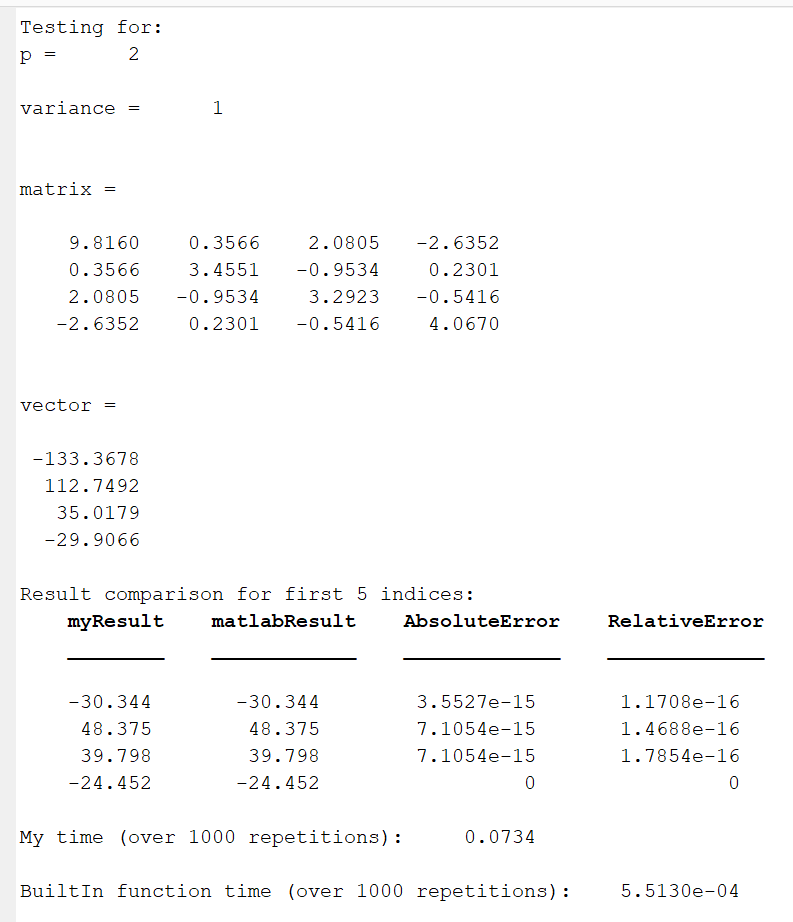
\includegraphics[width=\linewidth]{img/fig1.png}
            \caption{Caption for the first figure}
        \end{subfigure}
        \hfill
        \begin{subfigure}{0.45\linewidth}
            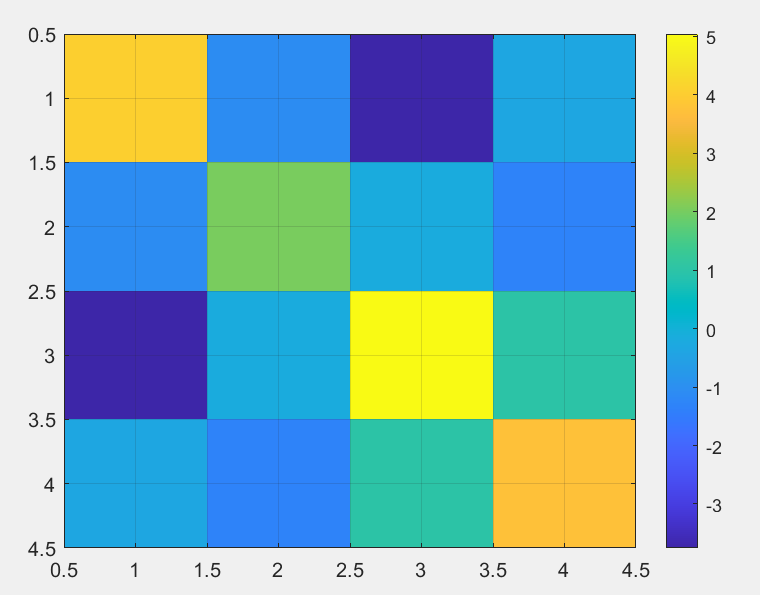
\includegraphics[width=\linewidth]{img/mat1.png}
            \caption{Caption for the second figure}
        \end{subfigure}

        \caption{$A1 \cdot x = b$}
        \label{fig:example1}
    \end{figure}
    
    \newpage
    \subsection*{Przykład 2}
    \vspace{12pt}
    \begin{figure}[hbt!]
        \centering

        \begin{subfigure}{0.45\linewidth}
            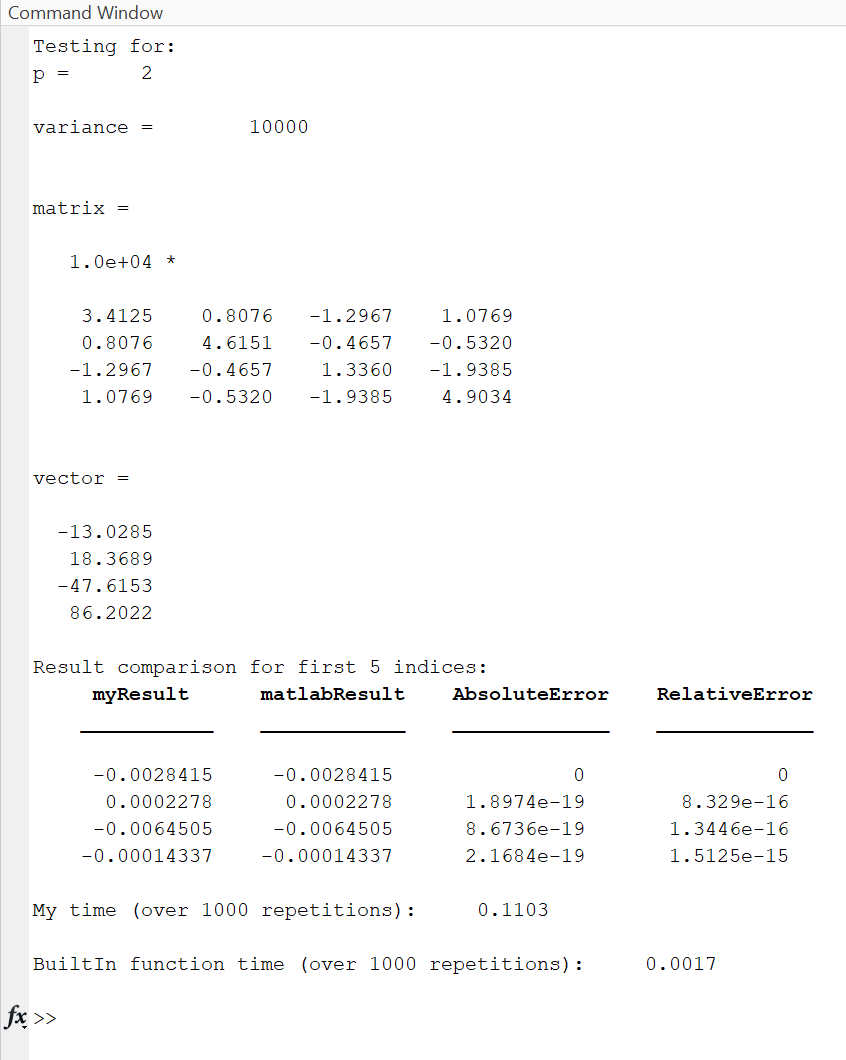
\includegraphics[width=\linewidth]{img/fig2.png}
            \caption{Caption for the first figure}
        \end{subfigure}
        \hfill
        \begin{subfigure}{0.45\linewidth}
            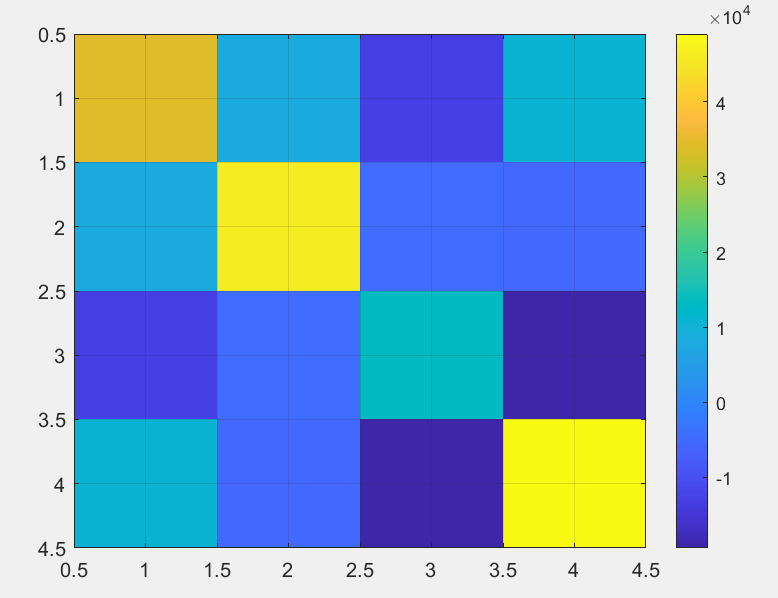
\includegraphics[width=\linewidth]{img/mat2.png}
            \caption{Caption for the second figure}
        \end{subfigure}

        \caption{$A1 \cdot x = b$}
        \label{fig:example2}
    \end{figure}
    
    \newpage
    \subsection*{Przykład 3}
    \vspace{12pt}
    \begin{figure}[hbt!]
        \centering

        \begin{subfigure}{0.45\linewidth}
            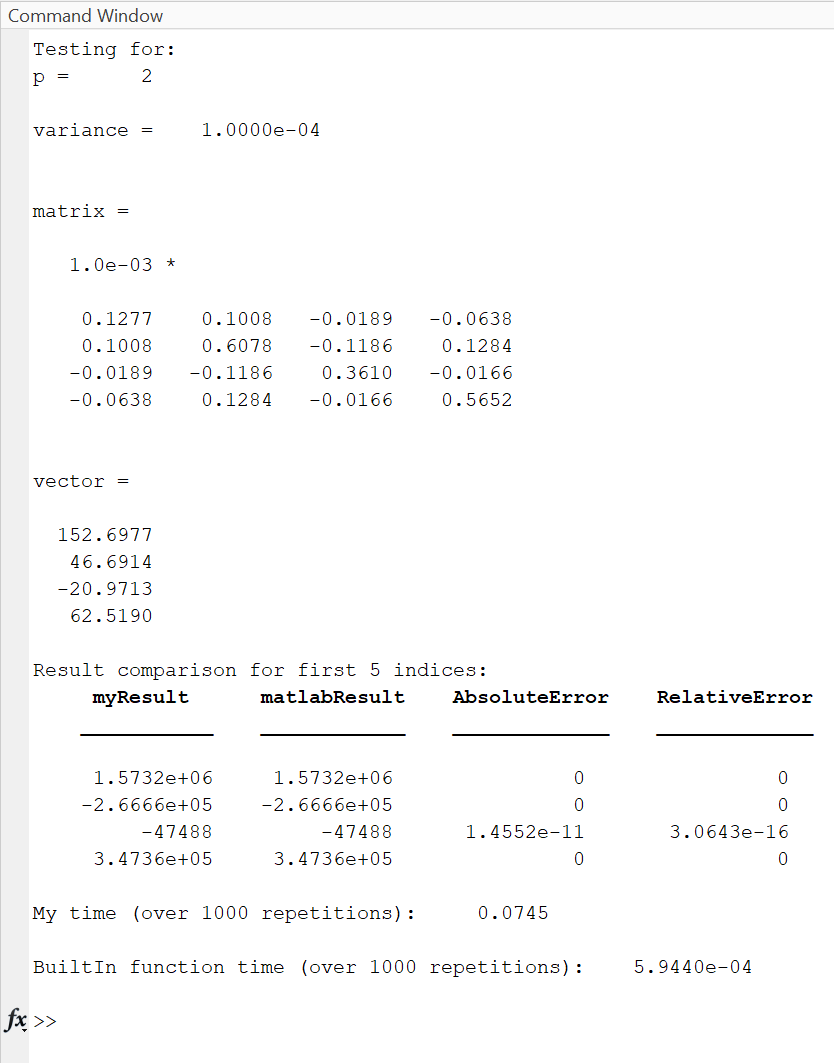
\includegraphics[width=\linewidth]{img/fig3.png}
            \caption{Caption for the first figure}
        \end{subfigure}
        \hfill
        \begin{subfigure}{0.45\linewidth}
            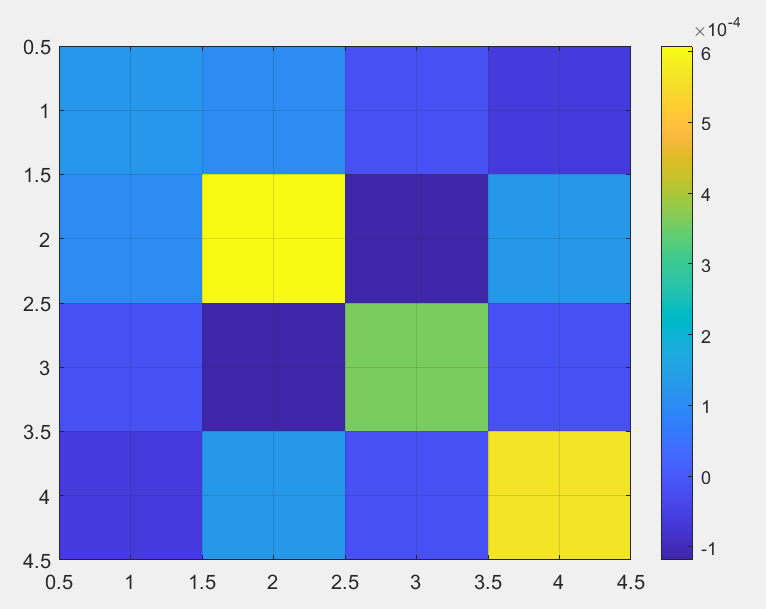
\includegraphics[width=\linewidth]{img/mat3.png}
            \caption{Caption for the second figure}
        \end{subfigure}

        \caption{$A1 \cdot x = b$}
        \label{fig:example3}
    \end{figure}
    
    \newpage
    \subsection*{Przykład 4}
    \vspace{12pt}
    \begin{figure}[hbt!]
        \centering

        \begin{subfigure}{0.45\linewidth}
            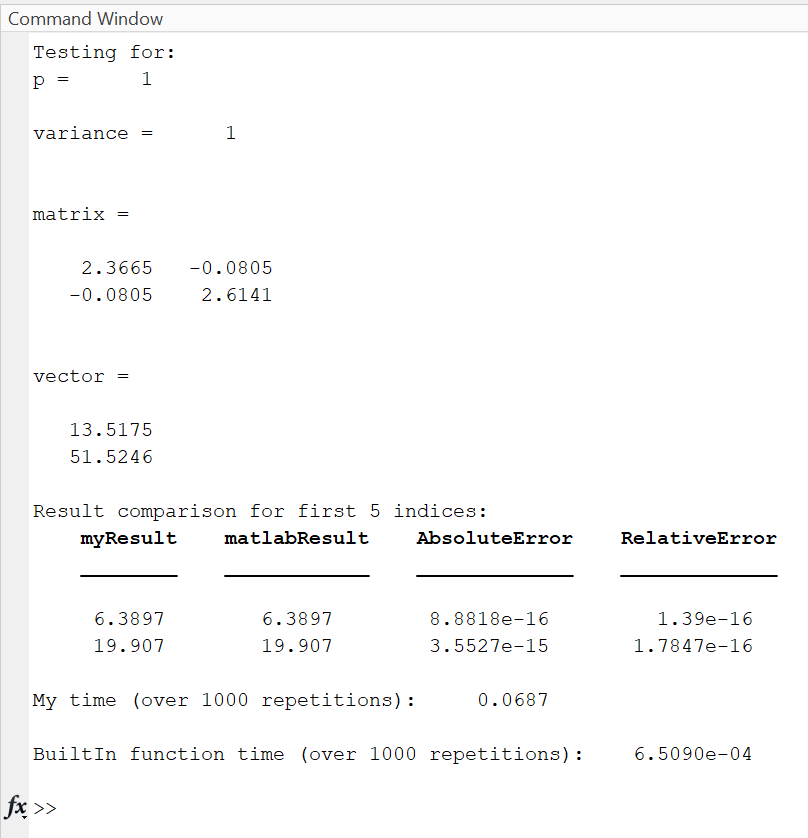
\includegraphics[width=\linewidth]{img/fig4.png}
            \caption{Caption for the first figure}
        \end{subfigure}
        \hfill
        \begin{subfigure}{0.45\linewidth}
            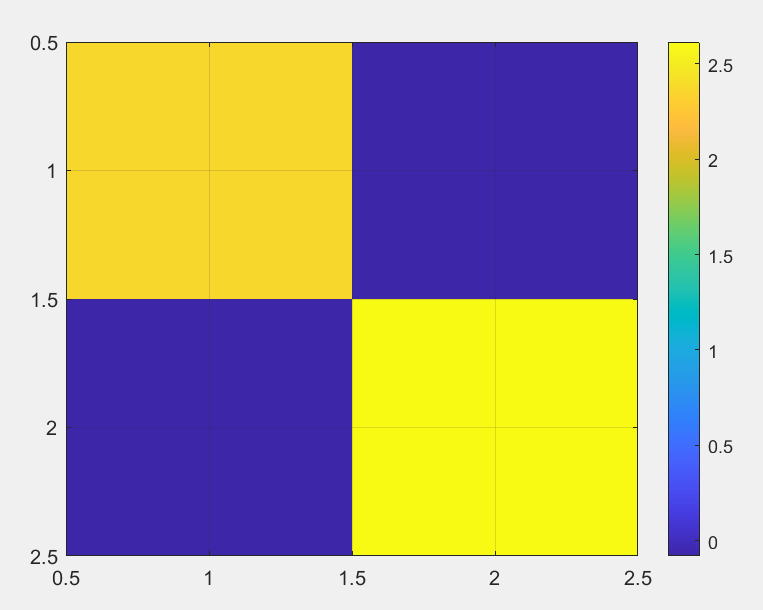
\includegraphics[width=\linewidth]{img/mat4.png}
            \caption{Caption for the second figure}
        \end{subfigure}

        \caption{$A1 \cdot x = b$}
        \label{fig:example4}
    \end{figure}
    
    \newpage
    \subsection*{Przykład 5}
    \vspace{12pt}
    \begin{figure}[hbt!]
        \centering

        \begin{subfigure}{0.45\linewidth}
            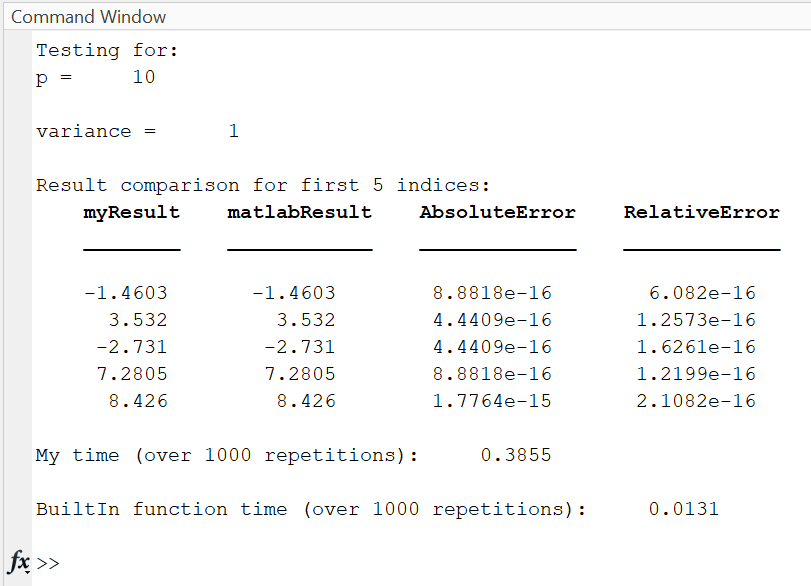
\includegraphics[width=\linewidth]{img/fig5.png}
            \caption{Caption for the first figure}
        \end{subfigure}
        \hfill
        \begin{subfigure}{0.45\linewidth}
            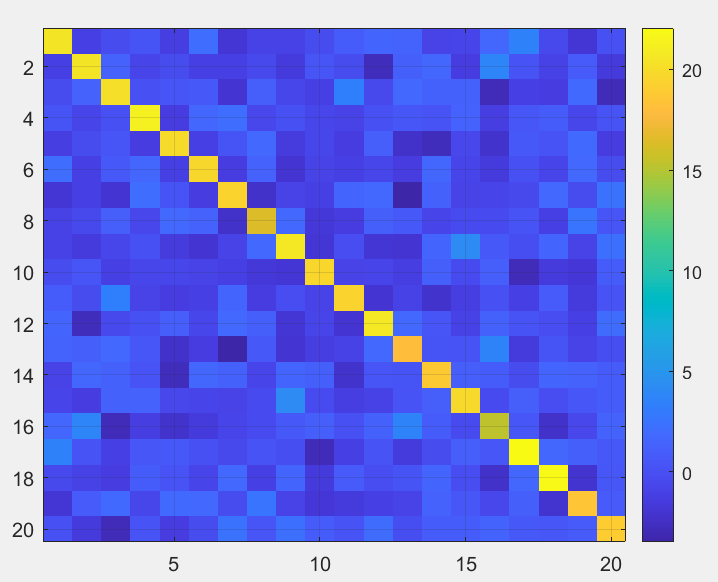
\includegraphics[width=\linewidth]{img/mat5.png}
            \caption{Caption for the second figure}
        \end{subfigure}

        \caption{$A1 \cdot x = b$}
        \label{fig:example5}
    \end{figure}
    
    \newpage
    \subsection*{Przykład 6}
    \vspace{12pt}
    \begin{figure}[hbt!]
        \centering

        \begin{subfigure}{0.45\linewidth}
            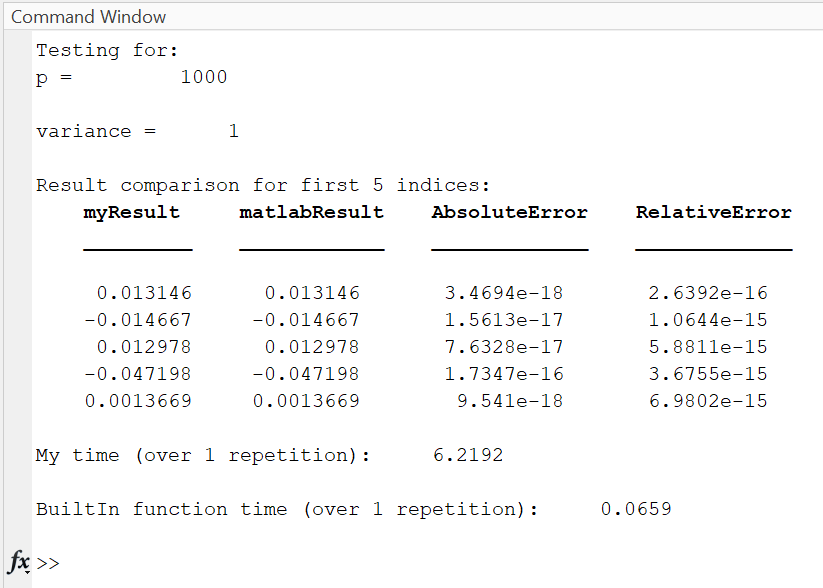
\includegraphics[width=\linewidth]{img/fig6.png}
            \caption{Caption for the first figure}
        \end{subfigure}
        \hfill
        \begin{subfigure}{0.45\linewidth}
            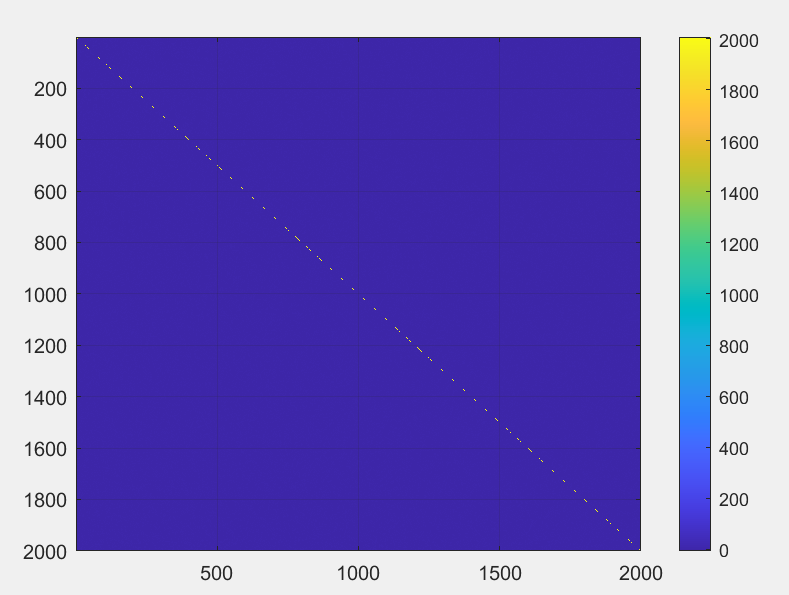
\includegraphics[width=\linewidth]{img/mat6.png}
            \caption{Caption for the second figure}
        \end{subfigure}

        \caption{$A1 \cdot x = b$}
        \label{fig:example6}
    \end{figure}
    
    \newpage
    \subsection*{Przykład 7}
    \vspace{12pt}
    \begin{figure}[hbt!]
        \centering

        \begin{subfigure}{0.45\linewidth}
            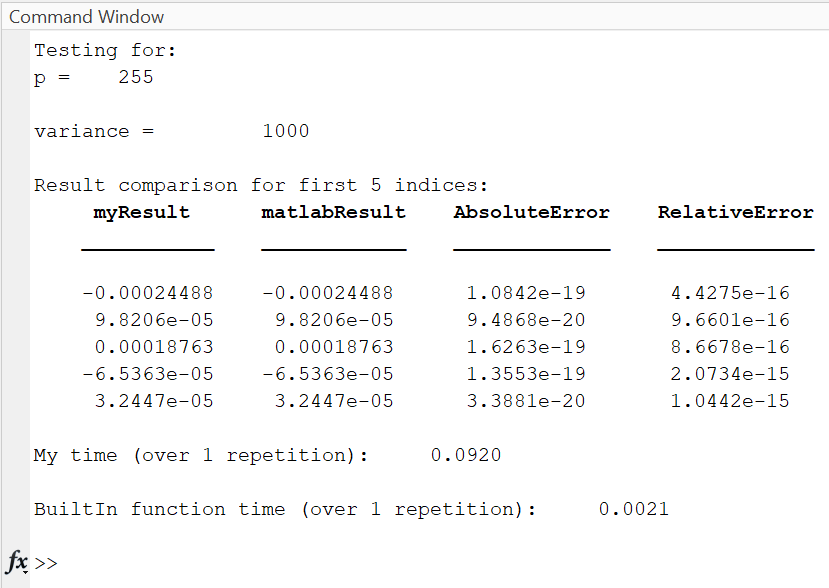
\includegraphics[width=\linewidth]{img/fig7.png}
            \caption{Caption for the first figure}
        \end{subfigure}
        \hfill
        \begin{subfigure}{0.45\linewidth}
            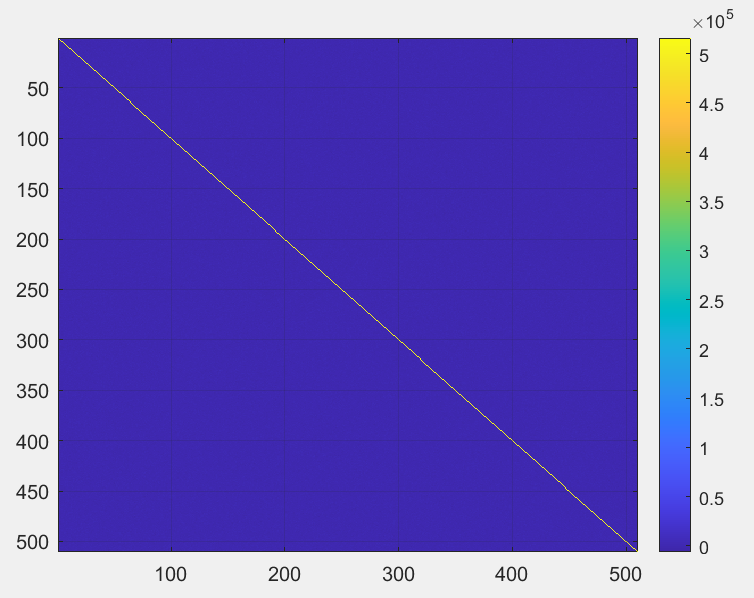
\includegraphics[width=\linewidth]{img/mat7.png}
            \caption{Caption for the second figure}
        \end{subfigure}

        \caption{$A1 \cdot x = b$}
        \label{fig:example7}
    \end{figure}
    
    \newpage
\end{document}

